% !TEX root = ../my-thesis.tex
%
\chapter{Fundamentals}
\label{sec:fundamentals}

This chapter aims to equip the reader with the mathematical and conceptual basics of particle-based fluid dynamics. We will introduce the underlying theory of Lagrangian fluid simulation and its physical relevance. Afterward, we explain how our representation of the fluid is generated and how it is stored in memory.

\section{Smoothed Particle Hydrodynamics}
\label{sec:sph}

The macroscopic real world we are seeing and experiencing every day is of continuous nature. Computers on the other hand are unable to capture this continuity reasonably. Thus, computer scientists have to invent ways of discretizing physical problems to be able to construct simulations for them. Smoothed Particle Hydrodynamics (SPH) is one such method of discretization. Originally invented for the simulation of gravitational systems in astronomy, it is now widely used in fluid simulation.

There are two prominent mathematical theories describing the computational simulation of hydrodynamics \cite{Monaghan:2005}: \\
In \textit{Eulerian} hydrodynamics, the fluid's properties are observed at fixed locations in space, usually arranged in a grid. This technique has built the foundation of computational fluid dynamics as we know it today. \\
In \textit{Lagrangian} hydrodynamics, the fluid's properties are carried through space by individual particles. These quantities are evaluated at the particles' freely moving positions instead of at fixed grid points.
Both methods are still in simultaneous use today as they differ in computational efficiency and physical accuracy. The choice of a best fit depends heavily on the application.

SPH belongs to the \textit{Lagrangian} category. The core idea is to approximate a continuous function $f$ with a finite set of particles $p_i$. Each particle consists of a position $\textbf{r}_i \in \mathbb{R}^3$ and an associated feature $f_i \in F$. Together, these form the set of particles $P := \{ p_i: i = 0,...,n-1 \}$ with $p_i := (\textbf{r}_i, f_i)$. Here, $F$ is a generic set of feature values that is dependent on the context of the problem. In the application discussed in this work, the feature of interest is the fluid's density. This can be represented by a scalar in $\mathbb{R}$, which is why we set $F := \mathbb{R}$. In other applications for example, it is common to see $F := \mathbb{R}^3$ and $f_i \in F$ to be interpreted as the particle's velocity (see Ummenhofer et al. \cite{Ummenhofer:2020}).

The continuous distribution of a feature in three-dimensional space is given by a function
\[
f: \mathbb{R}^3 \rightarrow F.
\]
Iterating over all particles $(\textbf{r}_i, f_i)$, $f$ can be approximated by the finite sum
\[
f(\textbf{r}) \approx \sum_{i=0}^{n-1} \space \frac{m_i}{\rho_i} \space f_i \space W(\textbf{r}_i - \textbf{r})
\]
where $W: \mathbb{R}^3 \rightarrow \mathbb{R}$ is called the \textit{smoothing kernel}, $\rho_i$ is the particle's density and $m_i$ is the particle's mass. In our case, the feature we are seeking to compute is the fluid's density $\rho$, so we set $f_i := \rho_i, \space i = 0,...,n-1$ and therefore - assuming all particles have identical mass $m$ - the equation simplifies to
\[
\rho(\textbf{r}) \approx m \sum_i W(\textbf{r}_i - \textbf{r}).
\]
Physically speaking, $\rho$ has the unit $\frac{\text{kg}}{\text{m}^3}$ meaning the kernel function $W$ has to have the unit $\text{m}^{-3}$.

\subsection{Surface definition}
\label{sec:surfacedefinition}

The fluid's surface $\mathcal{S}$ is defined as an iso-surface of the scalar field $\rho(\textbf{r})$. It is the set of all points where the evaluated density equals a constant we call $\sigma$:
\[
\mathcal{S} := \{ \textbf{r} \in \mathbb{R}^3 : \rho(\textbf{r}) = \sigma \}
\]
This definition is implied in algorithm 1 of Wu et al. \cite{Wu:2022} and is the basis for the surface extraction algorithm described later (see the chapter \textbf{Surface extraction with ray marching \myref{sec:surfaceextraction}}).

\subsection{Smoothing kernels}

\begin{figure}[h]
    \centering
    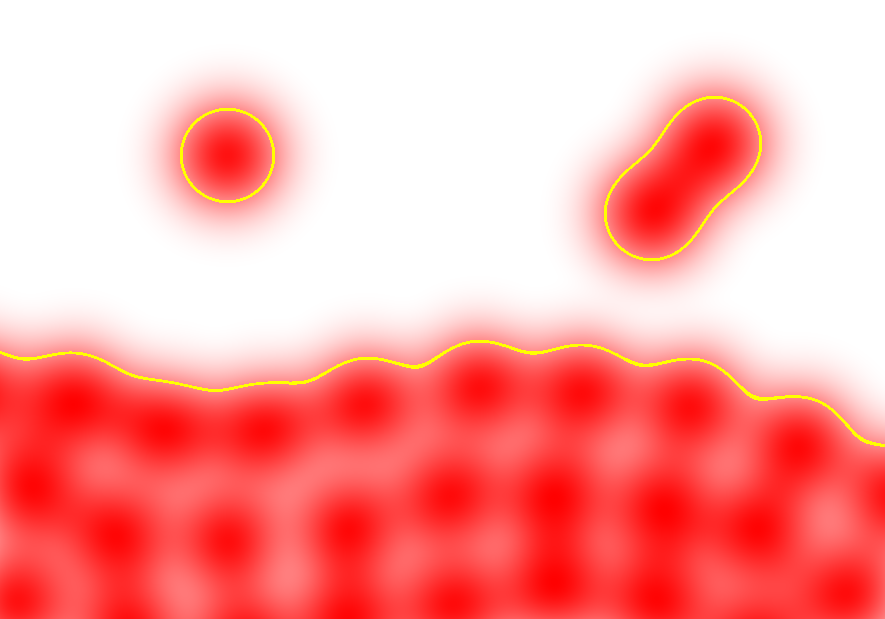
\includegraphics[width=0.75\textwidth]{my-gfx/figure-sph.png}
    \caption{An illustration showing how the kernel smoothes the particles' features across its neighborhood. The iso-surface $\mathcal{S}$ is indicated in yellow. The distinction between splash particles (top) and aggregated particles (bottom) can be seen and is important in later chapters.}
    \label{fig:sph}
\end{figure}

The kernel can be interpreted as a function that "smears" or smoothes the particles' features across space to create a continuum (see Figure \myref{fig:sph}). It must have some properties to function properly:

\begin{enumerate}
    \item Its volume integral over the entire domain is normalized (see \cite{Monaghan:2005}). This ensures that the kernel does not amplify the feature the particle is carrying:
    \[
    \int_{\mathbb{R}^3} W(\textbf{r}) \space d \textbf{r}' = 1
    \]
    
    \item It approaches the Dirac delta distribution for small support $h$ (explained below) (see \cite{Monaghan:2005}):
    \[
    \lim\limits_{h \rightarrow 0} W(\textbf{r}) = \delta(\textbf{r})
    \]
\end{enumerate}

For simulation, kernels are typically radially symmetric, meaning
\[ |\textbf{r}_1| = |\textbf{r}_2| \Rightarrow W(\textbf{r}_1) = W(\textbf{r}_2) .\]
However, this property is not always desired for this application for reasons explained in a later chapter.

The choice of a kernel function is important for error considerations and practicality. The authors did not state the specific function they used - only that it was a "symmetric decaying spline with finite support". In the following, the kernel definition by Koschier et al. \cite{Koschier:2019} will be used (see Figure \myref{fig:kernel}):

Let $r := \frac{|\textbf{r}|}{h}$:
\[
W(\textbf{r}) = c \frac{1}{h^3} P(r)
\]
where $c$ is a constant that satisfies the kernel's normalization constraint (for three dimensions $c := \frac{8}{\pi}$), $h$ is the particles' radius, and $P$ is a spline of the form
\[
P(r) = \begin{cases}
  6 (r^3 - r^2) + 1 , & 0 \leq r < \frac{1}{2} \\
  2 (1 - r)^3       , & \frac{1}{2} \leq r < 1 \\
  0                 , & \text{else.}
\end{cases}
\]
In this thesis, kernel functions $W$ are always understood with respect to the particle radius $h$ without stating so explicitly.

Note that this function is in fact radially symmetric, although we mentioned this to be an undesired property. It is used as the basis for a non-symmetric kernel later on.
These are some of the reasons for choosing this function:
\begin{itemize}
    \item It is simple and quick to compute.
    \item It has finite support, meaning $W(\textbf{r}) = 0, \forall \textbf{r}: |\textbf{r}| \geq h$. This opens the door for reducing the algorithm's time complexity, which is explained in the chapter \textbf{Particle neighborhood and anisotropic kernels \myref{sec:particleneighborhood}}.
\end{itemize}

\begin{figure}[h]
    \centering
    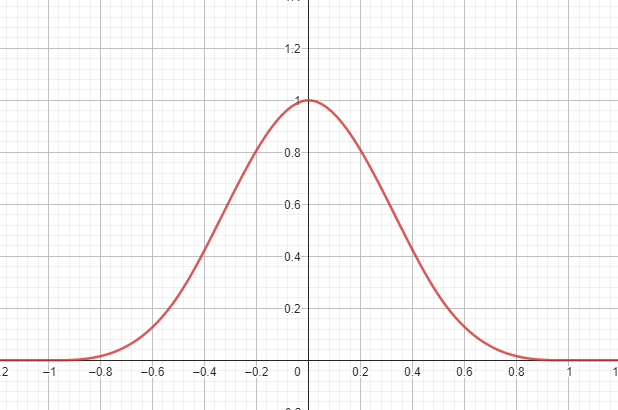
\includegraphics[width=0.75\textwidth]{my-gfx/figure-kernel.png}
    \caption{A graph showing the smoothing kernel we used. Here, only the spline $P$ is shown. The rest of $W$ consists only of scaling.}
    \label{fig:kernel}
\end{figure}


\subsection{Spatial derivative of the smoothing kernel}

The kernel function above is constructed in a way to be differentiable. The first spatial derivative $\nabla W$ is also continuous and smooth. It can be algebraically determined from the formula and implemented in a function directly, with no need to approximate it using numerical differentiation. $\nabla W$ will be used for calculating a normal vector of the fluid surface later on.

\subsection{Implementation}

What follows is the C++ code of our kernel function. It is based on the code of our fellow student Julian von Bülow. It is time-critical as it is evaluated thousands of times per frame. Hence, we made some small alterations to Julian's code to improve performance by a small margin. The full kernel code can be found in the file \textit{Kernel.cpp}.

\begin{lstlisting}[language=C++, caption={The implemented smoothing kernel function}\label{lst:smoothingkernel}]
float CubicSplineKernel::W(const glm::vec3& r_)
{
	float r = glm::dot(r_, r_);

	if (r >= h_squared)
		return 0.0f;

	r = glm::sqrt(r) * h_inv;
	
	if (r >= 0.5f)
	{
		const float q = 1.0f - r;
		return c * (2.0f * q * q * q);
	}
	
	return c * (6.0f * (r * r * r - r * r) + 1.0f);
}
\end{lstlisting}

These are the optimizations applied:
\begin{itemize}
    \item Line 6: Return from the function as soon as possible to avoid the expensive root computation.
    \item Line 8: Avoid divisions and instead pre-compute an inverse \textit{h\_inv} which can be used as a factor.
    \item A possible but not yet implemented improvement: Reduce the number of operations by using $c' := 2c$ instead of $c$.
\end{itemize}

\section{Datasets}
\label{sec:datasets}

\subsection{Particle representation}

The internal data representation for a particle is simply a vector of three 4-byte floating-point values containing its three-dimensional position. All particles are stored in an array consecutively. We had to be wary of memory alignment in C++ as structures are typically padded with unused memory to make their size a multiple of 16 bytes. Since a particle occupies only 12 bytes of memory, we tell the compiler not to optimize the memory alignment to prevent sacrificing a third of the necessary space. This decision has to be reevaluated when attempting to port the algorithm to the GPU as the preferred memory alignment varies from device to device. It is probably wise to keep the padding bytes and align the particles in chunks of 16 bytes to make memory access for modern hardware as streamlined as possible.

Memory alignment is a complicated topic and we did not have the time to measure the performance of different alignment strategies, although it would be very interesting to see if the speed of the program would be affected by this.

\subsection{Dataset generation}

Thanks to the simple particle representation, datasets can be generated in a variety of ways. The generator merely has to output particle positions for selected steps of the simulation. This strongly decouples the visualization from the underlying simulation. In fact, the data does not have to be computed using an SPH approach at all.

The library we used to generate datasets is the \textit{SPlisHSPlasH} framework developed by Jan Bender \cite{SplishSplash} which exports into the BGEO file format - a compressed binary format for storing geometry data used by a program called \textit{Houdini}. These files can then be imported into our program with the help of the \textit{Partio} library developed at the Walt Disney Animation Studios \cite{Partio}. It handles the decompression and reading of particle data for us.

When generating datasets, a range of parameters can be set to alter the physical interactions between particles like viscosity and particle mass. Some aspects of the simulation also affect the visualization, which is why each dataset needs some parameters in addition to the particle positions:
\begin{enumerate}
    \item The number of particles may vary. Many small particles can be used instead of fewer large particles to represent an identical fluid but with more detail. Therefore, the particles' mass has to be taken into consideration when determining the iso-surface density $\sigma$.
    \item Simulation is usually translation- and scale-invariant, meaning some datasets could have a larger spatial extent than others. As a solution, one can either set the ray marching step length to a fraction of the particles' size or scale the data to attain a specified average distance to neighboring particles.
\end{enumerate}

\subsection{Datasets used}


\begin{figure*}[h]
    \centering
    \begin{subfigure}[b]{0.475\textwidth}
        \centering
        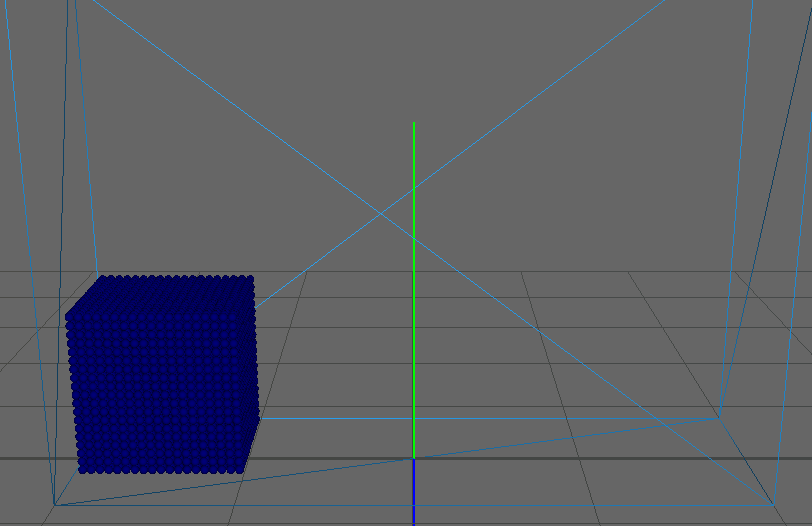
\includegraphics[width=\textwidth]{my-gfx/figure-dataset-1.png}  
    \end{subfigure}
    \hfill
    \begin{subfigure}[b]{0.475\textwidth}  
        \centering
        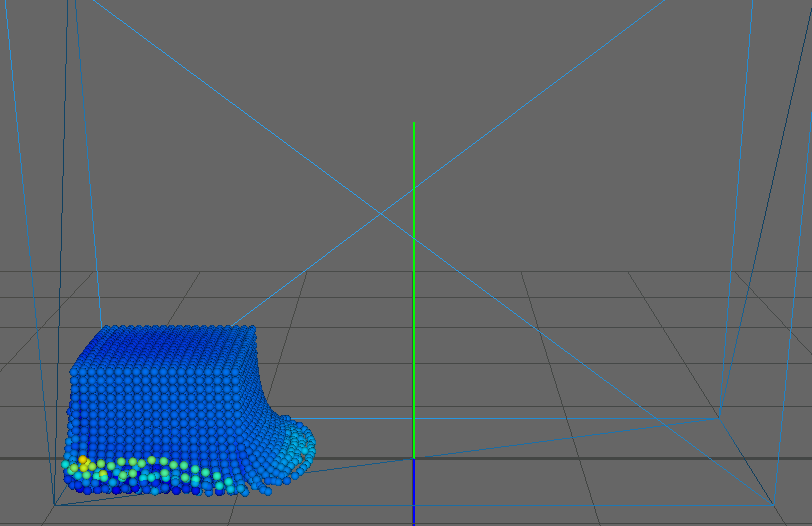
\includegraphics[width=\textwidth]{my-gfx/figure-dataset-2.png} 
    \end{subfigure}
    \vskip\baselineskip
    \begin{subfigure}[b]{0.475\textwidth}   
        \centering
        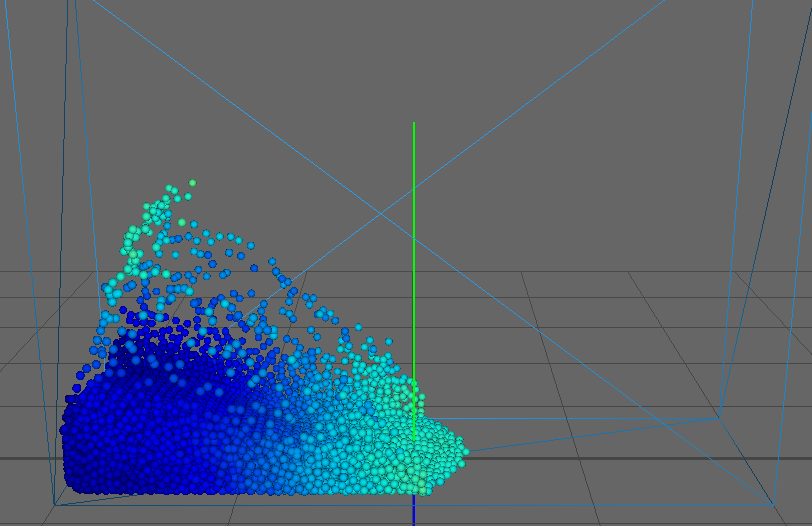
\includegraphics[width=\textwidth]{my-gfx/figure-dataset-3.png}  
    \end{subfigure}
    \hfill
    \begin{subfigure}[b]{0.475\textwidth}   
        \centering
        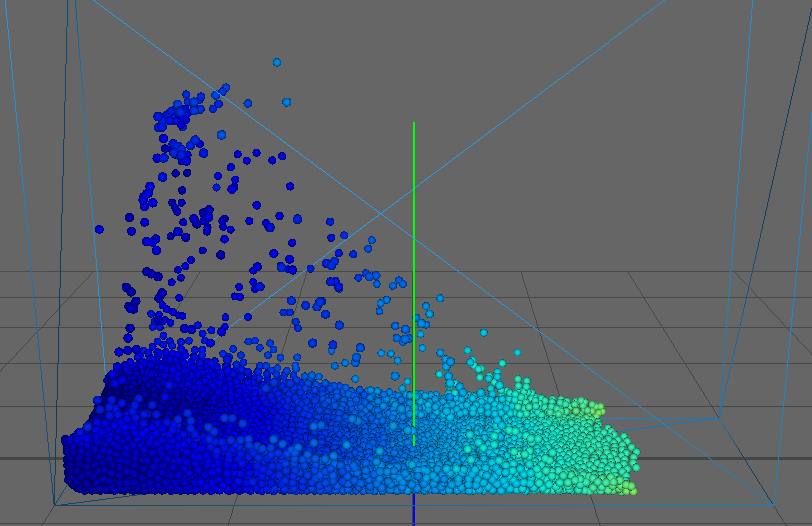
\includegraphics[width=\textwidth]{my-gfx/figure-dataset-4.png}
    \end{subfigure}
    
    \caption{Four simulation steps of our dataset: A cube of fluid dropping into a box (a so-called dam break scenario). Screenshots from the \textit{SPlisHSPlasH} application. The color gradient indicates the particles' velocity from low (blue) to high (green).}
    \label{fig:dataset}
\end{figure*}

As our main dataset for tests we used a typical dam break scenario, characterized by a block of fluid that drops into a confined box (Figure \myref{fig:dataset}). This frequently used dataset qualifies perfectly for our application as it features flat surfaces at the start (the block of fluid) and intricate edges and splashes as the block collides with the box, flinging into the air on the other side. We ran the simulation for about $10$ seconds, producing $123$ frames with $6859$ particles each.
